\subsection{Subsystem Decomposition} \label{subsection:subsystem_decomposition}

This subsection is a concretion of the system overview seen in Figure \ref{fig:flops_structure_overview}.
Decomposing an extensive system into its sub-components provides new insights and improves comprehension of the system.
The general approach for this endeavor is to use a UML component diagram.
It analyses if the system follows the open-closed principle of good software design.
This principle states that a system should "stay open for extension, but closed for modification" \cite{book:bruegge}.
To achieve this the system should strive for minimizing coupling and maximizing cohesion.
Cohesion expresses how tightly components of the same subsystem work together.
Coupling describes how components from different subsystems directly depend on each other without utilizing unifying interfaces, access points, or facades.

\begin{figure}[p]
    \begin{adjustwidth}{-0.175\paperwidth}{-0.175\paperwidth}
        \centering
        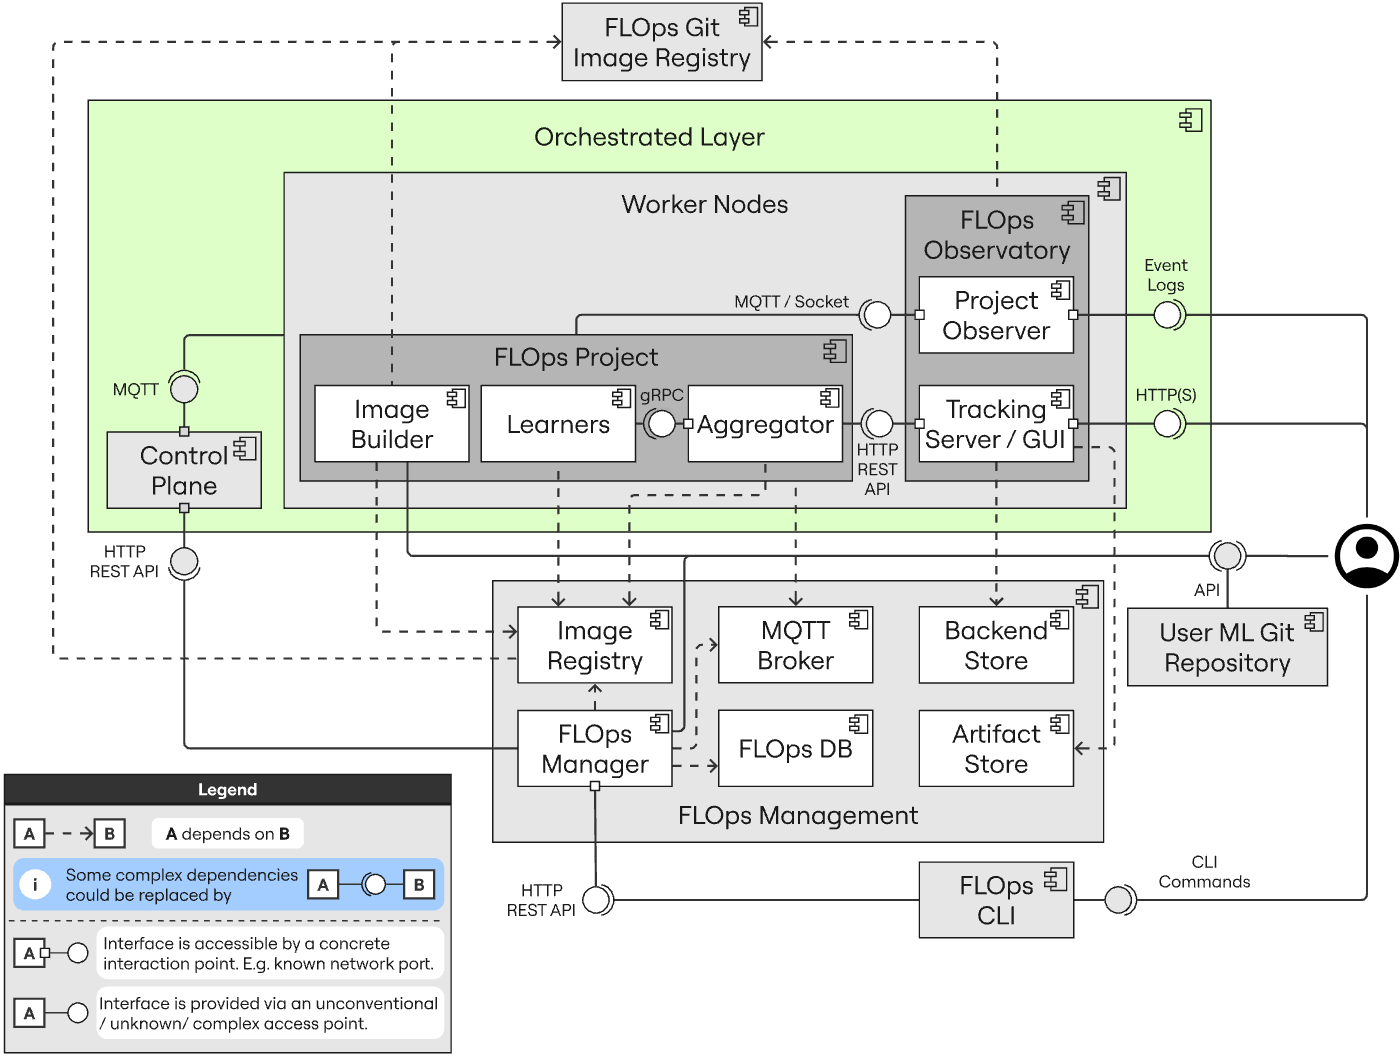
\includegraphics[width=0.975\paperwidth]{uml_component_diagram_overview.png}
        \caption{FLOps Subsystem Decomposition}
        \label{fig:component_diagram_overview}
    \end{adjustwidth}
\end{figure}

Figure \ref{fig:component_diagram_overview} shows a UML component diagram of the major FLOps components and subsystems.
The largest subsystems are the orchestrated layer and the FLOps management.
The FLOps management consists of six components.
The backend and artifact stores keep training metrics and models, respectively.
They are MLflow components.
The FLOps database stores all persistent information about FLOps' projects, components, apps, and services.
Note that this database is cleared when the management suite is restarted unlike the MLOps storages that are persistent across management restarts.
This simplifies state management and can be modified in the future.
The FLOps manager coordinates all FLOps processes.
These processes include serving a RESTful API for user requests, coordinating deployments with the orchestrator, checking requirements via its image registry, and accessing the user's repository.
The manager is the most important and largest part of the FLOps management suite.
The MQTT broker enables lightweight communication between the manager and deployed FLOps services.
The FLOps image registry provides complete control and direct access to images built by the image builder services.

The orchestrated layer contains the control plane and the worker nodes.
The control plane is independent of FLOps.
Only the FLOps manager interacts with it via its REST API.
The control plane resolves the FLOps management requests and creates, (un)deploys, or deletes components necessary for FLOps to run.
The relevant apps and services for FLOps are deployed on single or multiple worker nodes.
The two key FLOps apps are the project and observatory.
All project services can share their status with the manager or project observer over MQTT or socket messages.
The three services are dependent on the FLOps image registry.
The image builder needs to push images to it, whereas the FL actors are pulled from it.
By default, the learners and aggregator(s) communicate via gRPC (Flower).
The observatory services are the project observer(s) and tracking server.
The tracking server hosts the HTTP-based GUI and is accessible through a REST API.
The aggregator sends its logged metrics and model over the tracking server to the management stores.
The user can interact with the system via the GUI or by accessing the project observer's event (logs) over the control plane API or FLOps CLI.

The management image registry, project image builder, and observatory services are pulled from FLOps' public git image registry \cite{flops_code}.